\documentclass[10pt,a4paper]{article}
\usepackage[margin=2cm]{geometry}
\usepackage{booktabs,graphicx,xcolor,hyperref,caption,array,adjustbox}
\usepackage[T1]{fontenc}
\usepackage{lmodern}
\hypersetup{pdftitle={NeSy-Dec on Java monoliths: evaluation and comparison with the state of the art},pdfauthor={},pdfcreator={pdflatex},colorlinks=true,linkcolor=black,urlcolor=black}
\setlength{\parskip}{0.45em}\setlength{\parindent}{0pt}
\captionsetup{font=small,labelfont=bf}
\begin{document}
{\Large\bfseries NeSy-Dec on Java monoliths: evaluation and comparison with the state of the art}\\[0.4em]
{\small Results of 3 November 2026, after the Java fact base gained cannot-link constraints (rule CL-SIBLING). Every number below is read from \texttt{results\_java/results/*.csv}; the full tables, run log and claim-to-file map are in \texttt{RESULTS.md}, \texttt{RUNS.md} and \texttt{VERIFICATION.md}.}
\section{Summary}
\begin{itemize}\setlength{\itemsep}{2pt}
\item \textbf{GraphRL-Dec is the only method of the comparison pool that respects every cannot-link constraint.} On the 3 apps that have them (acmeair, daytrader7, lit-jpetstore), none of its 72 runs places a cannot-link pair in one service. Every other method of the pool violates pairs on at least one of these apps; rule-based repairs inside the same mask also comply, so the compliance comes from the mask (Section~\ref{sec:cl}).
\item \textbf{GraphRL-Dec is its teacher, repaired where the constraints forbid it.} On the 3 apps without cannot-link pairs, 72 of 72 runs decode to exactly the RoR-MSI teacher's partition; on the 3 apps with pairs, 0 of 72 do. Within our pipeline, GraphRL-Dec or its teacher has the highest composite Score on 5 of the 6 apps (Eq.~5, \texttt{evaluate.py} metrics), GraphRL-Dec alone on 3.
\item \textbf{Against the published tools} (Weerasinghe et al.\ 2026, Table~1), our best row is ranked \#1 of 15 on DayTrader, \#2 of 15 on AcmeAir, \#1 of 14 on JPetStore, \#1 of 15 on Plants when SM is computed on weighted calls, and \#5 of 15 on DayTrader, \#7 of 15 on AcmeAir, \#3 of 14 on JPetStore, \#7 of 15 on Plants when SM is binarized as in Sellami's code. The comparison is indicative only (Section~\ref{sec:threats}).
\item \textbf{NeSy-Rep fine-tuning improves the embeddings:} NeSy-Rep + Ward has a higher SM than pretrained UnixCoder + Ward on 6 of the 6 apps.
\item \textbf{Ablations.} Without the KL anchor it beats the teacher in 9 of 12 cases on the metric its reward uses, but in only 6 of 12 under the binarized metric; without the behaviour-cloning warm start it beats the teacher in 0 of 12.
\item \textbf{Sellami's HierDec and RLDec at their defaults do poorly on our graph}: HierDec fragments each app into many small services, RLDec's own decode returns one service on every app and seed.
\item \textbf{The Eq.~5 comparison can be gamed.} A hill-climb on SM, IFN, ICP and NED that starts from a \emph{random} partition, with no architectural knowledge, ranks \#1 in the published pool in 18 of 18 runs when SM counts weighted calls (Section~\ref{sec:after}). Rankings against published tools on these metrics are therefore not evidence of better decompositions, ours included. The same partitions violate cannot-link constraints; GraphRL-Dec's do not.
\item \textbf{A reward that is not the evaluation metric did not help GraphRL-Dec} (measured before the constraints were added): the dual reward beats the teacher on a held-out convention in fewer runs than the original reward.
\end{itemize}
\section{Setup}
Six subjects: the four benchmarks of Weerasinghe et al.\ in the repositories their footnotes link, plus the two versions the copied rows of their Table~1 were actually measured on (KimJongSung/jPetStore and the pbw-monolith, here \emph{lit-jpetstore} and \emph{lit-pbw}). Our analyzer (JavaParser 3.26.2 with a full classpath) resolves every call site except AcmeAir's proprietary wxs module; the layered resolver builds the graph $G$ every method partitions.
\begin{center}\resizebox{\ifdim\width>\linewidth\linewidth\else\width\fi}{!}{\begin{tabular}{lllrr}
\toprule
app & benchmark & version set & classes partitioned & edges in $G$ \\
\midrule
jpetstore-6 & JPetStore & footnote & 24 & 55 \\
acmeair & AcmeAir & both & 70 & 264 \\
daytrader7 & DayTrader & both & 104 & 299 \\
plantsbywebsphere & Plants & footnote & 35 & 101 \\
lit-jpetstore & JPetStore & literature & 71 & 219 \\
lit-pbw & Plants & literature & 36 & 100 \\
\bottomrule
\end{tabular}}\end{center}
Metrics are SM, IFN, ICP and NED, combined with Weerasinghe's Eq.~5 in the form that reproduces their published Score column exactly (sample standard deviation, divided by 7; 35 of 35 cells). Because the published rows come from several papers' own metric code, our rows are scored in two conventions: \emph{weighted calls} (Eq.~1--4 on our call graph) and \emph{binarized SM} (Sellami's RLDec metric code, which counts distinct dependencies). Within our pipeline the primary convention is \texttt{evaluate.py}'s, on $G$.
\section{Comparison with the state of the art}\label{sec:sota}
Each benchmark's pool is the published tools of Weerasinghe Table~1 (their metric values copied exactly) plus our rows; Eq.~5 is recomputed over the pool. Published rows marked $^\dagger$ were run by Weerasinghe et al.; the others were copied by them from the original papers. JPetStore and Plants use the literature versions. Figures~\ref{fig:sota} and~\ref{fig:sotab} show the two conventions; the tables give the weighted-call convention with the binarized rank beside it.
\begin{figure}[p]\centering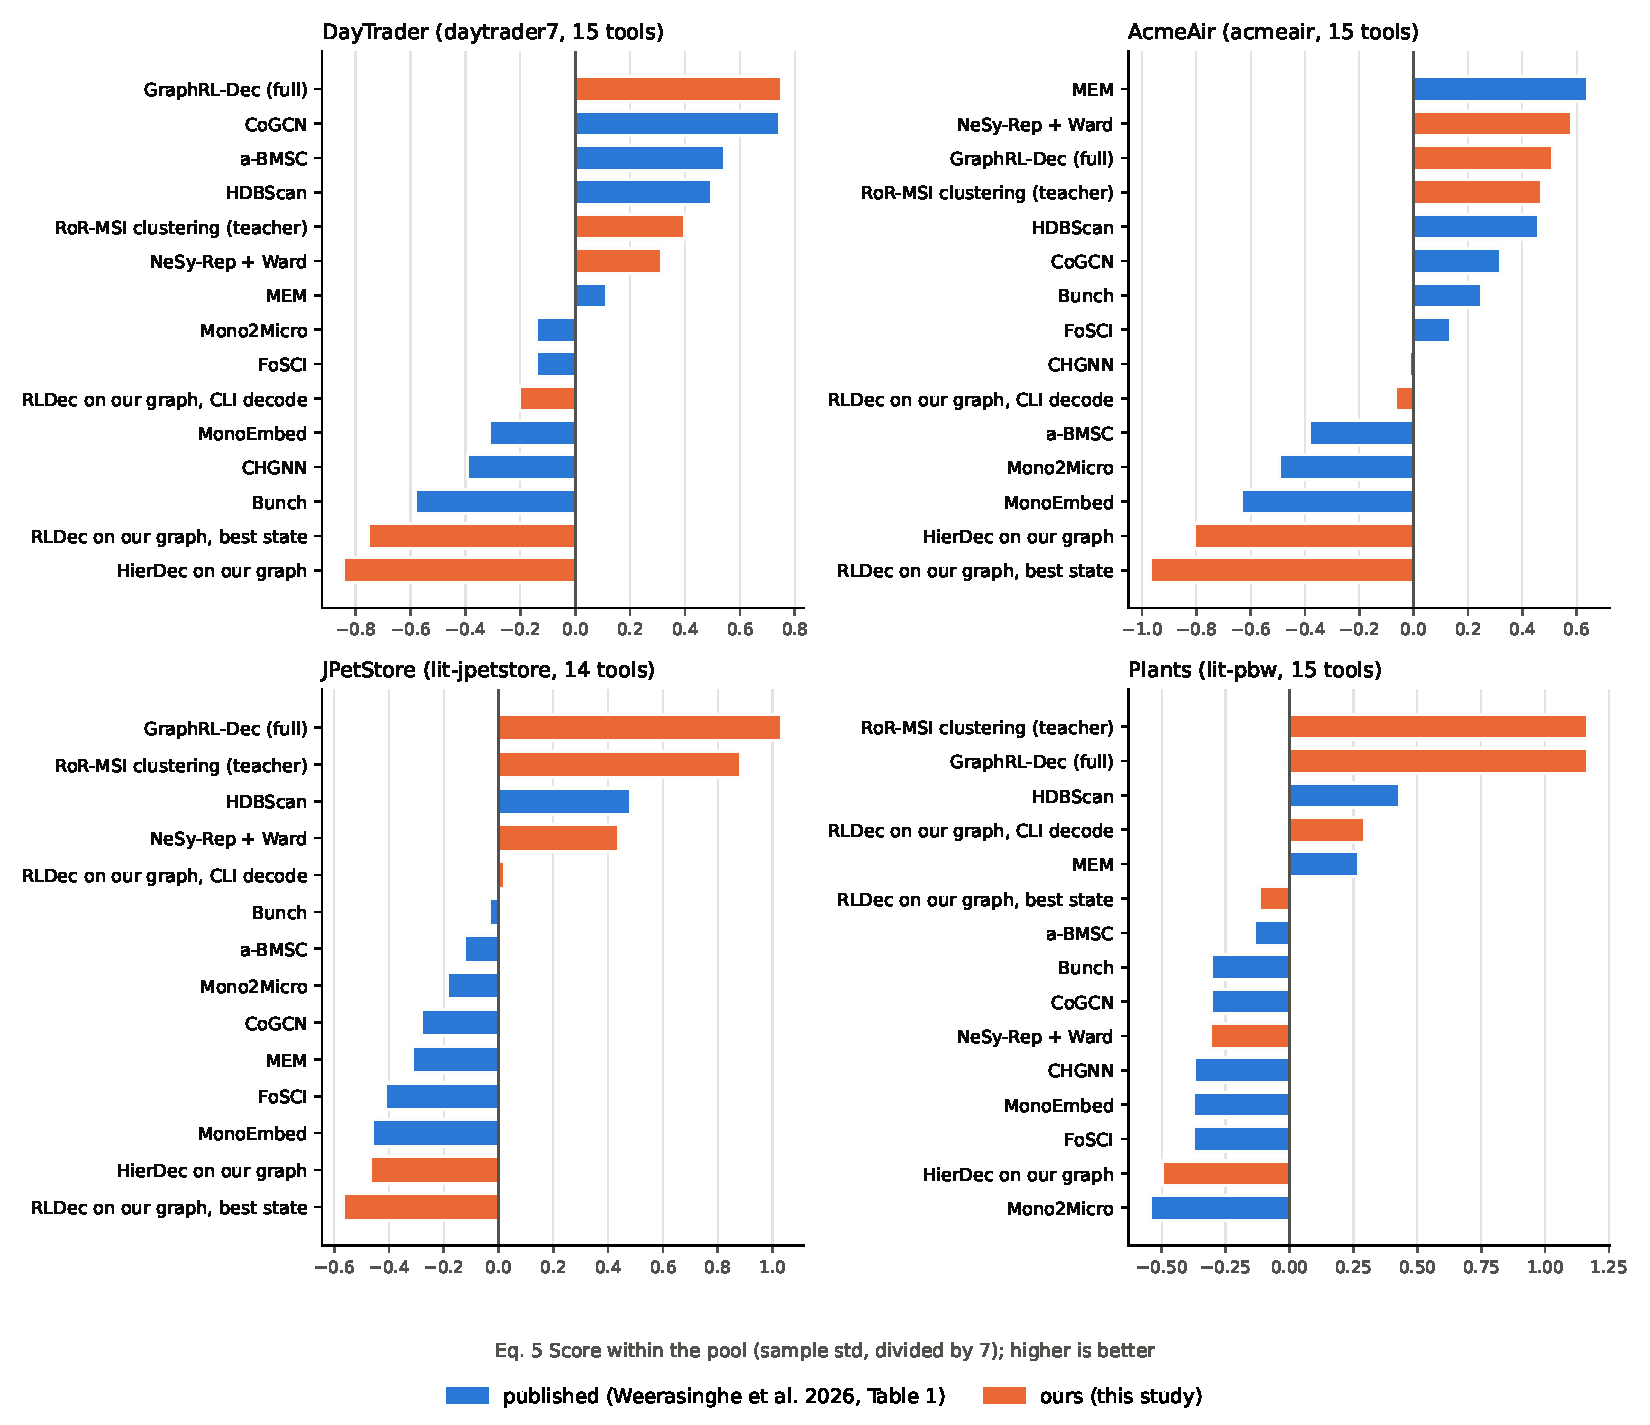
\includegraphics[width=\textwidth]{fig_sota_weighted.pdf}\caption{Eq.~5 Score of every tool in each benchmark's pool, our rows scored with SM on weighted calls (Weerasinghe Eq.~1--4). Orange: ours, on our graph; blue: published rows.}\label{fig:sota}\end{figure}
\begin{figure}[p]\centering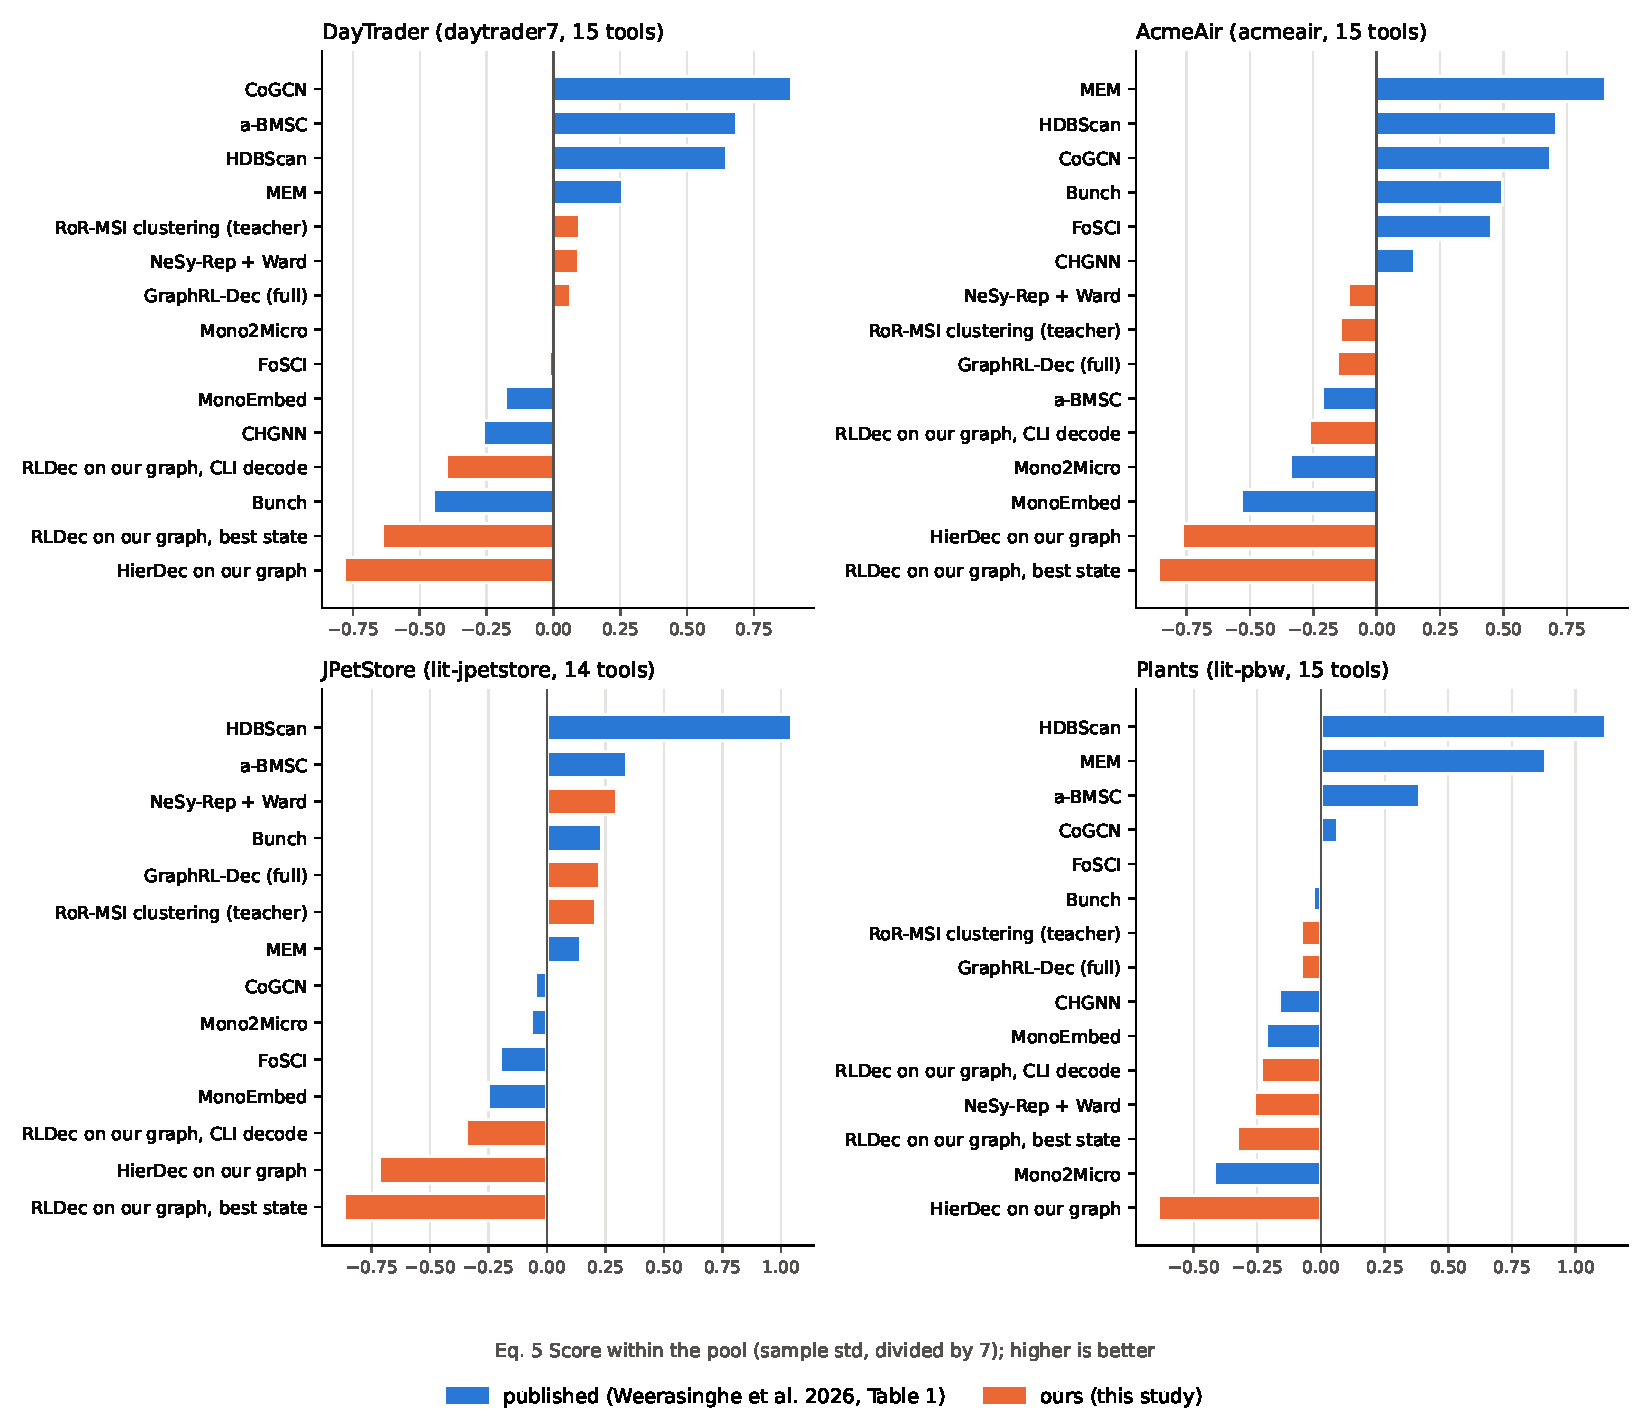
\includegraphics[width=\textwidth]{fig_sota_binarized.pdf}\caption{The same pools with our rows scored with binarized SM (Sellami's RLDec metric code).}\label{fig:sotab}\end{figure}
\subsection*{DayTrader (daytrader7, 104 classes)}
\begin{center}\small\resizebox{\ifdim\width>\linewidth\linewidth\else\width\fi}{!}{\begin{tabular}{rllrrrrrrr}
\toprule
rank & tool & source & SM & IFN & ICP & NED & published Score & pool Score & rank, binarized \\
\midrule
\textbf{1} & \textbf{GraphRL-Dec (full)} & \textbf{ours} & \textbf{0.44} & \textbf{2.27} & \textbf{0.34} & \textbf{0.55} & \textbf{--} & \textbf{+0.75} & \textbf{\#7} \\
2 & CoGCN & published & 0.49 & 3.00 & 0.35 & 0.70 & +0.73 & +0.74 & \#1 \\
3 & a-BMSC & published & 0.43 & 1.20 & 0.63 & 0.65 & +0.49 & +0.55 & \#2 \\
4 & HDBScan & published & 0.30 & 0.05 & 0.05 & 0.70 & +0.47 & +0.50 & \#3 \\
\textbf{5} & \textbf{RoR-MSI clustering (teacher)} & \textbf{ours} & \textbf{0.31} & \textbf{2.27} & \textbf{0.27} & \textbf{0.55} & \textbf{--} & \textbf{+0.40} & \textbf{\#5} \\
\textbf{6} & \textbf{NeSy-Rep + Ward} & \textbf{ours} & \textbf{0.25} & \textbf{2.00} & \textbf{0.47} & \textbf{0.27} & \textbf{--} & \textbf{+0.31} & \textbf{\#6} \\
7 & MEM & published & 0.32 & 3.50 & 0.25 & 0.95 & +0.04 & +0.11 & \#4 \\
8 & Mono2Micro & published & 0.08 & 1.92 & 0.35 & 0.34 & $-$0.15 & $-$0.14 & \#8 \\
9 & FoSCI & published & 0.30 & 7.00 & 0.82 & 0.55 & $-$0.17 & $-$0.14 & \#9 \\
\textbf{10} & \textbf{RLDec on our graph, CLI decode} & \textbf{ours} & \textbf{0.12} & \textbf{0.00} & \textbf{0.00} & \textbf{1.00} & \textbf{--} & \textbf{$-$0.20} & \textbf{\#12} \\
11 & MonoEmbed$^\dagger$ & published & 0.13 & 1.35 & 0.59 & 0.66 & $-$0.40 & $-$0.31 & \#10 \\
12 & CHGNN$^\dagger$ & published & 0.13 & 5.70 & 0.55 & 0.50 & $-$0.42 & $-$0.39 & \#11 \\
13 & Bunch & published & 0.18 & 11.00 & 0.50 & 0.65 & $-$0.58 & $-$0.58 & \#13 \\
\textbf{14} & \textbf{RLDec on our graph, best state} & \textbf{ours} & \textbf{0.01} & \textbf{2.22} & \textbf{0.86} & \textbf{0.54} & \textbf{--} & \textbf{$-$0.75} & \textbf{\#14} \\
\textbf{15} & \textbf{HierDec on our graph} & \textbf{ours} & \textbf{0.06} & \textbf{0.40} & \textbf{0.91} & \textbf{0.97} & \textbf{--} & \textbf{$-$0.84} & \textbf{\#15} \\
\bottomrule
\end{tabular}}\end{center}
\subsection*{AcmeAir (acmeair, 70 classes)}
\begin{center}\small\resizebox{\ifdim\width>\linewidth\linewidth\else\width\fi}{!}{\begin{tabular}{rllrrrrrrr}
\toprule
rank & tool & source & SM & IFN & ICP & NED & published Score & pool Score & rank, binarized \\
\midrule
1 & MEM & published & 0.30 & 0.70 & 0.05 & 0.38 & +0.69 & +0.64 & \#1 \\
\textbf{2} & \textbf{NeSy-Rep + Ward} & \textbf{ours} & \textbf{0.50} & \textbf{3.27} & \textbf{0.45} & \textbf{0.45} & \textbf{--} & \textbf{+0.58} & \textbf{\#7} \\
\textbf{3} & \textbf{GraphRL-Dec (full)} & \textbf{ours} & \textbf{0.44} & \textbf{3.45} & \textbf{0.45} & \textbf{0.27} & \textbf{--} & \textbf{+0.51} & \textbf{\#9} \\
\textbf{4} & \textbf{RoR-MSI clustering (teacher)} & \textbf{ours} & \textbf{0.42} & \textbf{3.45} & \textbf{0.45} & \textbf{0.27} & \textbf{--} & \textbf{+0.47} & \textbf{\#8} \\
5 & HDBScan & published & 0.30 & 0.30 & 0.02 & 0.90 & +0.53 & +0.46 & \#2 \\
6 & CoGCN & published & 0.42 & 0.90 & 0.60 & 1.00 & +0.46 & +0.32 & \#3 \\
7 & Bunch & published & 0.25 & 1.50 & 0.45 & 0.30 & +0.24 & +0.25 & \#4 \\
8 & FoSCI & published & 0.33 & 1.60 & 0.65 & 0.70 & +0.19 & +0.14 & \#5 \\
9 & CHGNN$^\dagger$ & published & 0.11 & 2.50 & 0.37 & 0.00 & $-$0.15 & $-$0.01 & \#6 \\
\textbf{10} & \textbf{RLDec on our graph, CLI decode} & \textbf{ours} & \textbf{0.08} & \textbf{0.00} & \textbf{0.00} & \textbf{1.00} & \textbf{--} & \textbf{$-$0.07} & \textbf{\#11} \\
11 & a-BMSC & published & 0.15 & 1.30 & 0.80 & 0.77 & $-$0.45 & $-$0.38 & \#10 \\
12 & Mono2Micro & published & 0.07 & 3.38 & 0.53 & 0.43 & $-$0.67 & $-$0.50 & \#12 \\
13 & MonoEmbed$^\dagger$ & published & 0.01 & 3.06 & 0.47 & 0.56 & $-$0.85 & $-$0.63 & \#13 \\
\textbf{14} & \textbf{HierDec on our graph} & \textbf{ours} & \textbf{$-$0.00} & \textbf{1.44} & \textbf{0.74} & \textbf{0.94} & \textbf{--} & \textbf{$-$0.81} & \textbf{\#14} \\
\textbf{15} & \textbf{RLDec on our graph, best state} & \textbf{ours} & \textbf{$-$0.01} & \textbf{4.08} & \textbf{0.79} & \textbf{0.55} & \textbf{--} & \textbf{$-$0.97} & \textbf{\#15} \\
\bottomrule
\end{tabular}}\end{center}
\subsection*{JPetStore (lit-jpetstore, 71 classes)}
\begin{center}\small\resizebox{\ifdim\width>\linewidth\linewidth\else\width\fi}{!}{\begin{tabular}{rllrrrrrrr}
\toprule
rank & tool & source & SM & IFN & ICP & NED & published Score & pool Score & rank, binarized \\
\midrule
\textbf{1} & \textbf{GraphRL-Dec (full)} & \textbf{ours} & \textbf{0.43} & \textbf{2.12} & \textbf{0.41} & \textbf{0.38} & \textbf{--} & \textbf{+1.03} & \textbf{\#5} \\
\textbf{2} & \textbf{RoR-MSI clustering (teacher)} & \textbf{ours} & \textbf{0.36} & \textbf{2.12} & \textbf{0.40} & \textbf{0.25} & \textbf{--} & \textbf{+0.88} & \textbf{\#6} \\
3 & HDBScan & published & 0.22 & 0.30 & 0.02 & 0.90 & +0.97 & +0.48 & \#1 \\
\textbf{4} & \textbf{NeSy-Rep + Ward} & \textbf{ours} & \textbf{0.29} & \textbf{3.00} & \textbf{0.61} & \textbf{0.12} & \textbf{--} & \textbf{+0.44} & \textbf{\#3} \\
\textbf{5} & \textbf{RLDec on our graph, CLI decode} & \textbf{ours} & \textbf{0.09} & \textbf{0.00} & \textbf{0.00} & \textbf{1.00} & \textbf{--} & \textbf{+0.02} & \textbf{\#12} \\
6 & Bunch & published & 0.10 & 2.70 & 0.00 & 0.38 & +0.05 & $-$0.03 & \#4 \\
7 & a-BMSC & published & 0.18 & 1.40 & 0.65 & 0.92 & +0.23 & $-$0.13 & \#2 \\
8 & Mono2Micro & published & 0.05 & 1.86 & 0.33 & 0.26 & $-$0.24 & $-$0.19 & \#9 \\
9 & CoGCN & published & 0.09 & 2.00 & 0.60 & 0.45 & $-$0.21 & $-$0.28 & \#8 \\
10 & MEM & published & 0.17 & 3.00 & 1.00 & 0.43 & +0.04 & $-$0.32 & \#7 \\
11 & FoSCI & published & 0.08 & 2.80 & 0.45 & 0.55 & $-$0.40 & $-$0.41 & \#10 \\
12 & MonoEmbed$^\dagger$ & published & 0.08 & 2.56 & 0.50 & 0.67 & $-$0.45 & $-$0.46 & \#11 \\
\textbf{13} & \textbf{HierDec on our graph} & \textbf{ours} & \textbf{0.08} & \textbf{0.61} & \textbf{0.82} & \textbf{0.94} & \textbf{--} & \textbf{$-$0.47} & \textbf{\#13} \\
\textbf{14} & \textbf{RLDec on our graph, best state} & \textbf{ours} & \textbf{0.08} & \textbf{2.23} & \textbf{0.75} & \textbf{0.72} & \textbf{--} & \textbf{$-$0.56} & \textbf{\#14} \\
\bottomrule
\end{tabular}}\end{center}
\subsection*{Plants (lit-pbw, 36 classes)}
\begin{center}\small\resizebox{\ifdim\width>\linewidth\linewidth\else\width\fi}{!}{\begin{tabular}{rllrrrrrrr}
\toprule
rank & tool & source & SM & IFN & ICP & NED & published Score & pool Score & rank, binarized \\
\midrule
\textbf{1} & \textbf{GraphRL-Dec (full)} & \textbf{ours} & \textbf{1.19} & \textbf{3.00} & \textbf{0.12} & \textbf{0.25} & \textbf{--} & \textbf{+1.17} & \textbf{\#8} \\
\textbf{2} & \textbf{RoR-MSI clustering (teacher)} & \textbf{ours} & \textbf{1.19} & \textbf{3.00} & \textbf{0.12} & \textbf{0.25} & \textbf{--} & \textbf{+1.17} & \textbf{\#7} \\
3 & HDBScan & published & 0.60 & 1.00 & 0.03 & 0.80 & +0.93 & +0.43 & \#1 \\
\textbf{4} & \textbf{RLDec on our graph, CLI decode} & \textbf{ours} & \textbf{0.47} & \textbf{0.00} & \textbf{0.00} & \textbf{1.00} & \textbf{--} & \textbf{+0.29} & \textbf{\#11} \\
5 & MEM & published & 0.54 & 3.30 & 0.22 & 0.25 & +0.71 & +0.27 & \#2 \\
\textbf{6} & \textbf{RLDec on our graph, best state} & \textbf{ours} & \textbf{0.33} & \textbf{1.65} & \textbf{0.21} & \textbf{0.90} & \textbf{--} & \textbf{$-$0.12} & \textbf{\#13} \\
7 & a-BMSC & published & 0.49 & 1.80 & 0.68 & 0.75 & +0.17 & $-$0.14 & \#3 \\
8 & Bunch & published & 0.22 & 5.50 & 0.30 & 0.10 & $-$0.18 & $-$0.30 & \#6 \\
9 & CoGCN & published & 0.33 & 3.50 & 0.55 & 0.50 & $-$0.13 & $-$0.30 & \#4 \\
\textbf{10} & \textbf{NeSy-Rep + Ward} & \textbf{ours} & \textbf{0.24} & \textbf{4.25} & \textbf{0.60} & \textbf{0.00} & \textbf{--} & \textbf{$-$0.31} & \textbf{\#12} \\
11 & CHGNN$^\dagger$ & published & 0.17 & 3.60 & 0.51 & 0.20 & $-$0.33 & $-$0.37 & \#9 \\
12 & MonoEmbed$^\dagger$ & published & 0.11 & 1.55 & 0.26 & 0.82 & $-$0.39 & $-$0.37 & \#10 \\
13 & FoSCI & published & 0.33 & 4.00 & 0.47 & 0.70 & $-$0.20 & $-$0.38 & \#5 \\
\textbf{14} & \textbf{HierDec on our graph} & \textbf{ours} & \textbf{0.26} & \textbf{0.90} & \textbf{0.80} & \textbf{0.95} & \textbf{--} & \textbf{$-$0.50} & \textbf{\#15} \\
15 & Mono2Micro & published & 0.08 & 6.00 & 0.38 & 0.04 & $-$0.57 & $-$0.54 & \#14 \\
\bottomrule
\end{tabular}}\end{center}
The footnote versions (mybatis/jpetstore-6 with 24 classes, WASdev Plants with 35) are smaller programs than the ones the published rows measured; their ranks in the same pools are:
\begin{center}\small\resizebox{\ifdim\width>\linewidth\linewidth\else\width\fi}{!}{\begin{tabular}{llrr}
\toprule
app & our row & rank, weighted calls & rank, binarized \\
\midrule
jpetstore-6 & RoR-MSI clustering (teacher) & \#3 of 14 & \#9 of 14 \\
jpetstore-6 & GraphRL-Dec (full) & \#2 of 14 & \#8 of 14 \\
jpetstore-6 & NeSy-Rep + Ward & \#1 of 14 & \#2 of 14 \\
plantsbywebsphere & RoR-MSI clustering (teacher) & \#2 of 15 & \#10 of 15 \\
plantsbywebsphere & GraphRL-Dec (full) & \#1 of 15 & \#11 of 15 \\
plantsbywebsphere & NeSy-Rep + Ward & \#7 of 15 & \#13 of 15 \\
\bottomrule
\end{tabular}}\end{center}
How to read this: on weighted calls our RoR-MSI-based rows lead or are near the top of every pool, but our weighted SM can exceed 1 (e.g.\ the teacher reaches 1.19 on lit-pbw) while no published SM exceeds 0.60, so this convention flatters weighted graphs. On binarized SM our rows fall to mid-table and a published row leads every pool (CoGCN on DayTrader, MEM on AcmeAir, HDBScan on JPetStore, HDBScan on Plants). The truth for a like-for-like comparison is unknown because the published numbers were computed with different code on different class sets.
\section{Within-pipeline comparison (same graph, same classes, same metric code)}
This is the fair comparison: every method partitions the same classes of the same graph, scored by one piece of code, with coverage 1.00 everywhere. Eq.~5 Score within each app's pool of nine methods; means over 3 seeds where a method has several runs.
\paragraph{Score, \texttt{evaluate.py} metrics on $G$ (primary).} Best per app in bold.
\begin{center}\small\resizebox{\ifdim\width>\linewidth\linewidth\else\width\fi}{!}{\begin{tabular}{lrrrrrr}
\toprule
method & jpetstore-6 & acmeair & daytrader7 & plantsbywebsphere & lit-jpetstore & lit-pbw \\
\midrule
RoR-MSI clustering (teacher) & +0.34 & +0.67 & +0.45 & \textbf{+0.85} & +0.60 & \textbf{+0.81} \\
GraphRL-Dec (full) & +0.34 & \textbf{+0.68} & \textbf{+0.74} & +0.85 & \textbf{+0.68} & +0.81 \\
NeSy-Rep + Ward & \textbf{+0.68} & +0.67 & +0.47 & +0.04 & +0.46 & +0.04 \\
UnixCoder + Ward & +0.26 & +0.11 & +0.12 & $-$0.70 & +0.28 & $-$0.64 \\
NeSy-Rep + HDBSCAN & +0.15 & $-$0.55 & +0.02 & +0.05 & $-$0.48 & $-$0.17 \\
HierDec on our graph & $-$0.67 & $-$0.54 & $-$0.44 & $-$0.40 & $-$0.44 & $-$0.32 \\
RLDec on our graph, CLI decode & +0.15 & +0.04 & $-$0.00 & +0.29 & +0.11 & +0.30 \\
RLDec on our graph, best state & $-$0.63 & $-$0.53 & $-$0.63 & $-$0.39 & $-$0.53 & $-$0.02 \\
random & $-$0.62 & $-$0.55 & $-$0.72 & $-$0.58 & $-$0.68 & $-$0.81 \\
\bottomrule
\end{tabular}}\end{center}
\paragraph{Score, binarized SM (RLDec's metric code) on $G$.} Best per app in bold.
\begin{center}\small\resizebox{\ifdim\width>\linewidth\linewidth\else\width\fi}{!}{\begin{tabular}{lrrrrrr}
\toprule
method & jpetstore-6 & acmeair & daytrader7 & plantsbywebsphere & lit-jpetstore & lit-pbw \\
\midrule
RoR-MSI clustering (teacher) & +0.20 & +0.61 & +0.59 & +0.49 & +0.54 & \textbf{+0.67} \\
GraphRL-Dec (full) & +0.20 & +0.59 & \textbf{+0.59} & +0.49 & +0.57 & +0.67 \\
NeSy-Rep + Ward & \textbf{+0.93} & \textbf{+0.69} & +0.44 & \textbf{+0.57} & \textbf{+0.63} & +0.37 \\
UnixCoder + Ward & +0.29 & +0.13 & +0.09 & $-$0.18 & +0.23 & $-$0.51 \\
NeSy-Rep + HDBSCAN & $-$0.09 & $-$0.39 & +0.07 & $-$0.06 & $-$0.42 & $-$0.09 \\
HierDec on our graph & $-$0.55 & $-$0.50 & $-$0.39 & $-$0.08 & $-$0.42 & $-$0.17 \\
RLDec on our graph, CLI decode & $-$0.09 & $-$0.11 & $-$0.18 & $-$0.33 & $-$0.03 & $-$0.22 \\
RLDec on our graph, best state & $-$0.38 & $-$0.44 & $-$0.55 & $-$0.01 & $-$0.54 & +0.08 \\
random & $-$0.51 & $-$0.59 & $-$0.66 & $-$0.90 & $-$0.55 & $-$0.80 \\
\bottomrule
\end{tabular}}\end{center}
\paragraph{Effect of NeSy-Rep fine-tuning.} SM of Ward clustering on pretrained against fine-tuned embeddings, same K:
\begin{center}\small\resizebox{\ifdim\width>\linewidth\linewidth\else\width\fi}{!}{\begin{tabular}{lrrrr}
\toprule
app & pretrained & NeSy-Rep & pretrained, binarized & NeSy-Rep, binarized \\
\midrule
jpetstore-6 & 0.70 & 0.93 & 0.11 & 0.19 \\
acmeair & 0.33 & 0.71 & 0.08 & 0.17 \\
daytrader7 & 0.35 & 0.47 & 0.10 & 0.14 \\
plantsbywebsphere & $-$0.24 & 0.69 & 0.04 & 0.09 \\
lit-jpetstore & 0.35 & 0.43 & 0.10 & 0.15 \\
lit-pbw & $-$0.22 & 0.60 & 0.01 & 0.12 \\
\bottomrule
\end{tabular}}\end{center}
\section{Constraint compliance (RQ4)}\label{sec:cl}
Java code has no namespace convention like the Rails one, so cannot-link comes from rule CL-SIBLING (\texttt{FACTS.md}, Section~2): two sibling packages are disjoint when each holds at least two active classes, no direct or type-use edge joins them, and they are peers, either in the same layer by stereotype or as alternative implementations of a common application interface. The rule fires on DayTrader (JSF front end against the servlet primitives and the WebSocket endpoints), AcmeAir (the MongoDB and eXtreme Scale back ends) and lit-jpetstore (the Spring MVC and Struts web layers). A violation is a pair placed in one service; means over seeds where a method has several runs:
\begin{center}\small\resizebox{\ifdim\width>\linewidth\linewidth\else\width\fi}{!}{\begin{tabular}{lrrr}
\toprule
method & acmeair (169 pairs) & daytrader7 (684 pairs) & lit-jpetstore (352 pairs) \\
\midrule
\textbf{GraphRL-Dec} & \textbf{0} & \textbf{0} & \textbf{0} \\
RoR-MSI (teacher) & 2 & 118 & 10 \\
NeSy-Rep + Ward & 11 & 32 & 0 \\
UnixCoder + Ward & 21 & 12 & 110 \\
HierDec & 13 & 0 & 18 \\
RLDec, best state & 25.7 & 42.0 & 52.7 \\
RLDec, CLI decode & 169 & 684 & 352 \\
random & 19.7 & 62.7 & 42.0 \\
\bottomrule
\end{tabular}}\end{center}
The RL environment masks every action that would place a class with a cannot-link partner, in training and in the decode, so GraphRL-Dec can violate a pair only through the mask's fallback, which makes every service legal when all are forbidden. In the variants with an outlier action, including \texttt{full}, one action always stays legal and a violation is impossible by construction; for all runs on these apps, a replay of the decode under the server's torch version reproduces every partition and shows the fallback never fired (\texttt{recon/mask\_replay.out}). The teacher does not see the constraints, and its violations are what the RL stage repairs: GraphRL-Dec moves only a few classes (\texttt{recon/graphrl\_repairs.out}). The repair raises SM, but partly by construction, because the rule separates packages with no edge between them in the graph SM is computed on. On daytrader7 it also costs must-link pairs: 24 of 41 are kept together, against the teacher's 30. The encoder's own cannot-link term barely acts (mean loss per epoch at most 0.00035, as in the Rails runs); the constraints reach the embeddings through the triplets.
\paragraph{Repair by rule.} Does the learned policy add anything over repairing the teacher by rule? Three rule-based repairs run in the same masked environment, with no learning: \texttt{repair\_masked} takes the teacher's service or the lowest-index legal one, \texttt{repair\_connect} the legal service with the most edge weight to the class, and \texttt{repair\_post} moves violating classes out of the teacher's finished partition. Each row takes GraphRL-Dec's place in the nine-method pool (GraphRL-Dec's own Score in brackets):
\begin{center}\small\resizebox{\ifdim\width>\linewidth\linewidth\else\width\fi}{!}{\begin{tabular}{llrrrrrrr}
\toprule
app & method & = GraphRL-Dec & moved & violations & must-link & Score & binarized & weighted calls \\
\midrule
acmeair & teacher & - & 0 & 2 of 169 & 0.538 & +0.67 (+0.68) & +0.61 (+0.59) & +0.64 (+0.66) \\
acmeair & graphrl:full & - & 2 / 2 / 2 & 0 of 169 & 0.538 & +0.68 (+0.68) & +0.59 (+0.59) & +0.66 (+0.66) \\
acmeair & repair\_masked & 0/3 & 2 & 0 of 169 & 0.538 & +0.67 (+0.68) & +0.58 (+0.59) & +0.64 (+0.66) \\
acmeair & repair\_connect & 0/3 & 2 & 0 of 169 & 0.538 & +0.68 (+0.68) & +0.60 (+0.59) & +0.66 (+0.66) \\
acmeair & repair\_post & 0/3 & 2 & 0 of 169 & 0.615 & +0.70 (+0.68) & +0.63 (+0.59) & +0.70 (+0.66) \\
daytrader7 & teacher & - & 0 & 118 of 684 & 0.732 & +0.54 (+0.74) & +0.60 (+0.59) & +0.57 (+0.80) \\
daytrader7 & graphrl:full & - & 21 / 21 / 21 & 0 of 684 & 0.585 & +0.74 (+0.74) & +0.59 (+0.59) & +0.80 (+0.80) \\
daytrader7 & repair\_masked & 0/3 & 14 & 0 of 684 & 0.585 & +0.77 (+0.74) & +0.60 (+0.59) & +0.83 (+0.80) \\
daytrader7 & repair\_connect & 0/3 & 14 & 0 of 684 & 0.585 & +0.76 (+0.74) & +0.59 (+0.59) & +0.83 (+0.80) \\
daytrader7 & repair\_post & 0/3 & 9 & 0 of 684 & 0.634 & +0.43 (+0.74) & +0.49 (+0.59) & +0.44 (+0.80) \\
lit-jpetstore & teacher & - & 0 & 10 of 352 & 0.568 & +0.64 (+0.68) & +0.55 (+0.57) & +0.75 (+0.81) \\
lit-jpetstore & graphrl:full & - & 5 / 5 / 5 & 0 of 352 & 0.568 & +0.68 (+0.68) & +0.57 (+0.57) & +0.81 (+0.81) \\
lit-jpetstore & repair\_masked & 0/3 & 5 & 0 of 352 & 0.568 & +0.66 (+0.68) & +0.53 (+0.57) & +0.81 (+0.81) \\
lit-jpetstore & repair\_connect & 0/3 & 5 & 0 of 352 & 0.568 & +0.66 (+0.68) & +0.55 (+0.57) & +0.79 (+0.81) \\
lit-jpetstore & repair\_post & 0/3 & 2 & 0 of 352 & 0.591 & +0.66 (+0.68) & +0.56 (+0.57) & +0.76 (+0.81) \\
\bottomrule
\end{tabular}}\end{center}
All repairs violate nothing, so compliance comes from the mask, not from the learning. The best repair matches GraphRL-Dec's quality: it is at most 0.02 below it anywhere and above it on AcmeAir and DayTrader. On these benchmarks the RL stage behaves as a learned constraint repair, and a rule does about as well.
\section{GraphRL-Dec and the ablation}
With the Rails settings (behaviour-cloning warm start from the teacher, KL anchor 0.5, PPO learning rate $10^{-4}$, 600 episodes), 72 of 144 runs (8 reward variants $\times$ 6 apps $\times$ 3 seeds) decode to exactly the teacher's partition, all of them on the apps without cannot-link pairs; on the others the action mask is what makes the policy deviate. Two labelled ablations (72 runs, with the same mask) test whether PPO can leave the teacher on its own. Each ablation row takes GraphRL-Dec's place in the nine-method pool.
\begin{center}\small\resizebox{\ifdim\width>\linewidth\linewidth\else\width\fi}{!}{\begin{tabular}{lllrrrr}
\toprule
app & ablation & variant & Score & teacher & Score, binarized & teacher, binarized \\
\midrule
jpetstore-6 & no KL, 2,000 ep. & structural & +0.57 & +0.29 & +0.38 & +0.17 \\
jpetstore-6 & no KL, 2,000 ep. & full & +0.52 & +0.29 & +0.32 & +0.18 \\
jpetstore-6 & no warm start & structural & +0.15 & +0.39 & $-$0.08 & +0.24 \\
jpetstore-6 & no warm start & full & +0.15 & +0.39 & $-$0.08 & +0.24 \\
acmeair & no KL, 2,000 ep. & structural & +0.65 & +0.68 & +0.54 & +0.62 \\
acmeair & no KL, 2,000 ep. & full & +0.66 & +0.67 & +0.48 & +0.64 \\
acmeair & no warm start & structural & $-$0.64 & +0.87 & $-$0.69 & +0.78 \\
acmeair & no warm start & full & $-$0.11 & +0.80 & $-$0.09 & +0.72 \\
daytrader7 & no KL, 2,000 ep. & structural & +0.81 & +0.36 & +0.20 & +0.73 \\
daytrader7 & no KL, 2,000 ep. & full & +0.89 & +0.33 & +0.66 & +0.54 \\
daytrader7 & no warm start & structural & $-$0.12 & +0.70 & $-$0.50 & +0.85 \\
daytrader7 & no warm start & full & $-$0.10 & +0.68 & $-$0.27 & +0.79 \\
plantsbywebsphere & no KL, 2,000 ep. & structural & +1.01 & +0.73 & +0.58 & +0.47 \\
plantsbywebsphere & no KL, 2,000 ep. & full & +1.01 & +0.74 & +0.58 & +0.48 \\
plantsbywebsphere & no warm start & structural & +0.35 & +1.03 & $-$0.26 & +0.55 \\
plantsbywebsphere & no warm start & full & +0.35 & +1.03 & $-$0.26 & +0.55 \\
lit-jpetstore & no KL, 2,000 ep. & structural & +0.76 & +0.55 & +0.43 & +0.57 \\
lit-jpetstore & no KL, 2,000 ep. & full & +0.75 & +0.58 & +0.64 & +0.52 \\
lit-jpetstore & no warm start & structural & $-$0.21 & +0.79 & $-$0.14 & +0.68 \\
lit-jpetstore & no warm start & full & +0.05 & +0.76 & $-$0.06 & +0.64 \\
lit-pbw & no KL, 2,000 ep. & structural & +0.77 & +0.83 & +0.51 & +0.73 \\
lit-pbw & no KL, 2,000 ep. & full & +0.84 & +0.78 & +0.30 & +0.78 \\
lit-pbw & no warm start & structural & +0.37 & +1.00 & $-$0.18 & +0.80 \\
lit-pbw & no warm start & full & +0.37 & +1.00 & $-$0.18 & +0.80 \\
\bottomrule
\end{tabular}}\end{center}
Without the anchor, PPO beats the teacher in 9 of 12 cases on \texttt{evaluate.py} metrics, which are the very functions its reward is built from, but in only 6 of 12 under the binarized metric. Without the warm start it collapses, mostly to a single service or to no assigned class at all. The RL stage therefore depends on the RoR-MSI teacher, and its unanchored gains transfer across metric conventions only in part.
\section{Follow-up: can the RL stage beat the rule?}
Two follow-up GPU experiments. First, GraphRL-Dec without the KL anchor and with 2,000 episodes (\emph{kl0}), a setting chosen beforehand on the three apps without cannot-link pairs only (\texttt{recon/setting\_selection.out}) and then applied unchanged. Second, GraphRL-Dec warm-started from NeSy-Rep + Ward instead of the RoR-MSI teacher, compared with rule-based repairs of that partition. Each row takes GraphRL-Dec's place in the nine-method pool:
\begin{center}\scriptsize\resizebox{\ifdim\width>\linewidth\linewidth\else\width\fi}{!}{\begin{tabular}{llrrrrrrr}
\toprule
app & method & runs & violations & must-link & semantic & Score & binarized & weighted calls \\
\midrule
acmeair & RoR-MSI teacher & 1 & 2 & 0.538 & 0.453 & +0.67 & +0.61 & +0.64 \\
acmeair & GraphRL-Dec full, paper setting & 3 & 0 & 0.538 & 0.432 & +0.68 & +0.59 & +0.66 \\
acmeair & best repair of the teacher (repair\_post) & 1 & 0 & 0.615 & 0.440 & +0.70 & +0.63 & +0.70 \\
acmeair & GraphRL-Dec full, kl0 & 3 & 0 & 0.564 & 0.406 & +0.66 & +0.48 & +0.65 \\
acmeair & GraphRL-Dec structural, kl0 & 3 & 0 & 0.538 & 0.417 & +0.65 & +0.54 & +0.61 \\
acmeair & NeSy-Rep + Ward & 1 & 11 & 0.615 & 0.634 & +0.66 & +0.65 & +0.68 \\
acmeair & best repair of NeSy-Rep + Ward (repair\_nesyward\_connect) & 1 & 0 & 0.615 & 0.564 & +0.71 & +0.67 & +0.74 \\
acmeair & GraphRL-Dec full from NeSy-Rep + Ward, paper setting & 3 & 0 & 0.615 & 0.564 & +0.33 & +0.56 & +0.24 \\
acmeair & GraphRL-Dec full from NeSy-Rep + Ward, kl0 & 3 & 0 & 0.641 & 0.457 & +0.41 & +0.27 & +0.30 \\
acmeair & GraphRL-Dec structural from NeSy-Rep + Ward, kl0 & 3 & 0 & 0.615 & 0.433 & +0.57 & +0.23 & +0.58 \\
daytrader7 & RoR-MSI teacher & 1 & 118 & 0.732 & 0.356 & +0.54 & +0.60 & +0.57 \\
daytrader7 & GraphRL-Dec full, paper setting & 3 & 0 & 0.585 & 0.435 & +0.74 & +0.59 & +0.80 \\
daytrader7 & best repair of the teacher (repair\_masked) & 1 & 0 & 0.585 & 0.419 & +0.77 & +0.60 & +0.83 \\
daytrader7 & GraphRL-Dec full, kl0 & 3 & 0 & 0.675 & 0.437 & +0.89 & +0.66 & +0.90 \\
daytrader7 & GraphRL-Dec structural, kl0 & 3 & 0 & 0.667 & 0.425 & +0.81 & +0.20 & +0.92 \\
daytrader7 & NeSy-Rep + Ward & 1 & 32 & 0.634 & 0.608 & +0.57 & +0.50 & +0.46 \\
daytrader7 & best repair of NeSy-Rep + Ward (repair\_nesyward\_post) & 1 & 0 & 0.683 & 0.590 & +0.55 & +0.50 & +0.38 \\
daytrader7 & GraphRL-Dec full from NeSy-Rep + Ward, paper setting & 3 & 0 & 0.683 & 0.591 & +0.56 & +0.49 & +0.40 \\
daytrader7 & GraphRL-Dec full from NeSy-Rep + Ward, kl0 & 3 & 0 & 0.683 & 0.594 & +0.56 & +0.50 & +0.40 \\
daytrader7 & GraphRL-Dec structural from NeSy-Rep + Ward, kl0 & 3 & 0 & 0.683 & 0.594 & +0.56 & +0.50 & +0.40 \\
lit-jpetstore & RoR-MSI teacher & 1 & 10 & 0.568 & 0.456 & +0.64 & +0.55 & +0.75 \\
lit-jpetstore & GraphRL-Dec full, paper setting & 3 & 0 & 0.568 & 0.453 & +0.68 & +0.57 & +0.81 \\
lit-jpetstore & best repair of the teacher (repair\_masked) & 1 & 0 & 0.568 & 0.437 & +0.66 & +0.53 & +0.81 \\
lit-jpetstore & GraphRL-Dec full, kl0 & 3 & 0 & 0.561 & 0.460 & +0.75 & +0.64 & +0.87 \\
lit-jpetstore & GraphRL-Dec structural, kl0 & 3 & 0 & 0.788 & 0.451 & +0.76 & +0.43 & +0.90 \\
lit-jpetstore & NeSy-Rep + Ward & 1 & 0 & 0.773 & 0.686 & +0.51 & +0.61 & +0.42 \\
lit-jpetstore & best repair of NeSy-Rep + Ward (repair\_nesyward\_masked) & 1 & 0 & 0.773 & 0.686 & +0.51 & +0.61 & +0.42 \\
lit-jpetstore & GraphRL-Dec full from NeSy-Rep + Ward, paper setting & 3 & 0 & 0.773 & 0.686 & +0.51 & +0.61 & +0.42 \\
lit-jpetstore & GraphRL-Dec full from NeSy-Rep + Ward, kl0 & 3 & 0 & 0.758 & 0.665 & +0.54 & +0.60 & +0.47 \\
lit-jpetstore & GraphRL-Dec structural from NeSy-Rep + Ward, kl0 & 3 & 0 & 0.788 & 0.672 & +0.55 & +0.62 & +0.47 \\
\bottomrule
\end{tabular}}\end{center}
Without the anchor, GraphRL-Dec beats the best rule-based repair on DayTrader and lit-jpetstore in all three conventions, but not on AcmeAir. Across all six apps and eight variants its gain over the paper setting is mostly in the reward's own metric family and transfers to binarized SM in under a third of the cases (\texttt{followup.md}, Table F2). The NeSy-Rep warm start does not help: it at best ties the repair of its own starting partition. Every new run on the constrained apps has zero violations.
\section{Experiments after the main run}\label{sec:after}
These ran on a local RTX 3060 (GraphRL-Dec) and CPU (the rest); the full account is \texttt{OPTIMIZATION.md}. They are labelled experiments and replace nothing above.
\paragraph{A reward that is not the evaluation metric.} Measured on 26 October 2026, before the fact base had cannot-link pairs, and not repeated. The dual reward averages the \texttt{evaluate.py} and binarized z-scores; the weighted-call convention is in neither term and serves as the held-out check. Runs beating the teacher, each seed scored alone in the nine-method pool:
\begin{center}\small\resizebox{\ifdim\width>\linewidth\linewidth\else\width\fi}{!}{\begin{tabular}{lrrr}
\toprule
setting & \texttt{evaluate.py} & binarized & held out \\
\midrule
dual reward, no anchor, full & 7/18 & 6/18 & 7/18 \\
dual reward, no anchor, structural & 8/18 & 6/18 & 5/18 \\
old reward, no anchor, full & 9/18 & 5/18 & 9/18 \\
old reward, no anchor, structural & 13/18 & 6/18 & 11/18 \\
dual reward, paper's anchor, full & 0/3 & 0/3 & 0/3 \\
\bottomrule
\end{tabular}}\end{center}
It does not make GraphRL-Dec better than the teacher across apps; on AcmeAir and DayTrader it returns to the teacher's exact partition in every run.
\paragraph{Hill-climbing the same objective.} A search that repeatedly applies the best single-class move (under the RL environment's size cap) beats the teacher on all six apps in all three conventions when started from the teacher. Started from random partitions it does as well, and in the published pools it ranks as follows (random partitions alone in columns 7 and 8; the last column counts the cannot-link pairs the hill-climbed partition violates):
\begin{center}\small\resizebox{\ifdim\width>\linewidth\linewidth\else\width\fi}{!}{\begin{tabular}{llrrrrrrr}
\toprule
app & benchmark & seed & services & weighted & binarized & random, weighted & random, binarized & cannot-link violated \\
\midrule
jpetstore-6 & JPetStore & 42 & 4 & \#1 of 9 & \#2 of 9 & \#7 of 9 & \#9 of 9 & no pairs \\
jpetstore-6 & JPetStore & 1 & 4 & \#1 of 9 & \#2 of 9 & \#9 of 9 & \#9 of 9 & no pairs \\
jpetstore-6 & JPetStore & 7 & 4 & \#1 of 9 & \#5 of 9 & \#1 of 9 & \#9 of 9 & no pairs \\
acmeair & AcmeAir & 42 & 11 & \#1 of 10 & \#6 of 10 & \#10 of 10 & \#10 of 10 & 17 of 169 \\
acmeair & AcmeAir & 1 & 11 & \#1 of 10 & \#7 of 10 & \#10 of 10 & \#10 of 10 & 16 of 169 \\
acmeair & AcmeAir & 7 & 11 & \#1 of 10 & \#7 of 10 & \#10 of 10 & \#10 of 10 & 8 of 169 \\
daytrader7 & DayTrader & 42 & 11 & \#1 of 10 & \#5 of 10 & \#10 of 10 & \#10 of 10 & 87 of 684 \\
daytrader7 & DayTrader & 1 & 11 & \#1 of 10 & \#5 of 10 & \#10 of 10 & \#10 of 10 & 91 of 684 \\
daytrader7 & DayTrader & 7 & 11 & \#1 of 10 & \#5 of 10 & \#9 of 10 & \#10 of 10 & 91 of 684 \\
plantsbywebsphere & Plants & 42 & 3 & \#1 of 10 & \#7 of 10 & \#10 of 10 & \#10 of 10 & no pairs \\
plantsbywebsphere & Plants & 1 & 3 & \#1 of 10 & \#7 of 10 & \#10 of 10 & \#10 of 10 & no pairs \\
plantsbywebsphere & Plants & 7 & 3 & \#1 of 10 & \#7 of 10 & \#9 of 10 & \#10 of 10 & no pairs \\
lit-jpetstore & JPetStore & 42 & 8 & \#1 of 9 & \#5 of 9 & \#9 of 9 & \#9 of 9 & 46 of 352 \\
lit-jpetstore & JPetStore & 1 & 8 & \#1 of 9 & \#3 of 9 & \#9 of 9 & \#9 of 9 & 63 of 352 \\
lit-jpetstore & JPetStore & 7 & 8 & \#1 of 9 & \#5 of 9 & \#9 of 9 & \#9 of 9 & 71 of 352 \\
lit-pbw & Plants & 42 & 4 & \#1 of 10 & \#7 of 10 & \#10 of 10 & \#10 of 10 & no pairs \\
lit-pbw & Plants & 1 & 4 & \#1 of 10 & \#7 of 10 & \#9 of 10 & \#10 of 10 & no pairs \\
lit-pbw & Plants & 7 & 4 & \#1 of 10 & \#9 of 10 & \#10 of 10 & \#10 of 10 & no pairs \\
\bottomrule
\end{tabular}}\end{center}
Some moves are sensible (on jpetstore-6, \texttt{Item} and \texttt{Product} join the catalog service), others are not (on DayTrader, benchmark servlets such as \texttt{PingJDBCRead} join the account-data service), and measures the search does not optimize (embedding similarity within services, must-link facts kept together) change only slightly. The gain is optimization of the metric family itself, so the refinement is not reported as a method. Cannot-link compliance tells it apart from an architecturally informed decomposition.
\paragraph{Why our rows rank lower under binarized SM.} Binarized SM is the dependency density inside each service (distinct internal edges divided by the squared size). Our graphs are sparse, a service of about nine classes has a density near 0.2, below a two-class service with one edge (0.25), and Eq.~5 weights SM three times, so tools emitting many tiny services gain (the published HDBScan row has NED 0.70--0.90 and SM up to 0.60). RLDec's code also counts self-calls, which our graph omits:
\begin{center}\small\resizebox{\ifdim\width>\linewidth\linewidth\else\width\fi}{!}{\begin{tabular}{lrrrrr}
\toprule
app & graph density & mean service size & density inside services & binarized SM & with self-calls \\
\midrule
lit-jpetstore & 0.043 & 8.9 & 0.191 & 0.17 & 0.20 \\
daytrader7 & 0.028 & 9.5 & 0.218 & 0.21 & 0.30 \\
acmeair & 0.054 & 6.4 & 0.251 & 0.21 & 0.23 \\
lit-pbw & 0.077 & 9.0 & 0.196 & 0.16 & 0.30 \\
\bottomrule
\end{tabular}}\end{center}
\paragraph{Resolver layers.} The teacher run on the naive declared-type graph cannot place the classes that graph leaves isolated; on the resolved graph it places all of them:
\begin{center}\small\resizebox{\ifdim\width>\linewidth\linewidth\else\width\fi}{!}{\begin{tabular}{lrrrrr}
\toprule
app & classes & unplaceable, naive graph & unplaceable, resolved graph & SM, naive & SM, resolved \\
\midrule
jpetstore-6 & 24 & 1 & 0 & 0.62 & 0.74 \\
acmeair & 70 & 21 & 0 & 0.17 & 0.65 \\
daytrader7 & 104 & 13 & 0 & 0.09 & 0.49 \\
plantsbywebsphere & 35 & 0 & 0 & 1.41 & 1.39 \\
lit-jpetstore & 71 & 7 & 0 & 0.16 & 0.46 \\
lit-pbw & 36 & 0 & 0 & 1.39 & 1.43 \\
\bottomrule
\end{tabular}}\end{center}
The SM column is computed on the resolved graph for both partitions, which favours the resolved one; the unplaceable counts do not depend on any metric.
\section{Where the study stands}
\textbf{Supported by the evidence:}
\begin{itemize}\setlength{\itemsep}{2pt}
\item the Java front end (analyzer, layered resolver with provenance, symbolic facts) works on all six subjects, and without the resolver a large share of classes cannot be placed at all;
\item NeSy-Rep fine-tuning improves the code embeddings;
\item Weerasinghe's published Score column is reproduced exactly only with sample standard deviation divided by 7, not with the formula in their text;
\item rankings on SM, IFN, ICP and NED flip with the SM definition, and a knowledge-free search tops every published tool, so these metrics cannot establish state-of-the-art decomposition quality;
\item GraphRL-Dec's action mask enforces the cannot-link constraints: it is the only method with no violation on every app that has them, and it repairs its teacher's violations with a few moves.
\end{itemize}
\textbf{Not supported:} that the learned policy adds quality over a rule-based repair of its teacher on Java; that GraphRL-Dec beats the published tools, since its SM gains over the teacher are partly built into the constraint rule and the metric comparison is gameable; that CL-SIBLING generalises, since it was written on these six subjects.

\textbf{Next step.} Evidence of decomposition quality needs a criterion no method optimizes: an expert or published reference decomposition for these applications, compared with agreement measures such as MoJoFM, and the cannot-link rule applied unchanged to Java systems it was not designed on.
\section{Threats to validity}\label{sec:threats}
\begin{itemize}\setlength{\itemsep}{2pt}
\item \textbf{Metric code.} The published rows were computed by several papers with their own code; three ICP definitions are in circulation and SM may or may not be weighted. Our two conventions bracket the plausible readings; neither is guaranteed to match.
\item \textbf{Class sets.} Our class counts differ from the published ones (DayTrader 104 against 118, AcmeAir 70 against 86, JPetStore 71 against 73, Plants 36 against 40), and how the papers counted nested and anonymous classes is not stated.
\item \textbf{Inputs.} All our methods are static; Mono2Micro and some others used execution traces.
\item \textbf{Copied numbers.} Only CHGNN and MonoEmbed were run by Weerasinghe et al.; the other published rows are copied from earlier papers.
\item \textbf{Baseline inputs.} HierDec and RLDec ran unmodified at their defaults on our graph, not on Sellami's analysis service; per-app tuning from their papers is not available. This is the fair within-pipeline comparison, not a reproduction of their papers.
\item \textbf{The cannot-link rule was written on these subjects} and fires on three of the six; it has not been applied to other Java systems.
\item \textbf{The rule and SM read the same graph}, so separating the rule's packages tends to raise SM; the compliance result itself does not depend on this.
\end{itemize}
\section{Reproducibility}
Rebuilding jpetstore-6 from source reproduces every CPU-stage output exactly, except for the order of tied triplets (Python hash randomisation in the shared triplet generator). Two GraphRL-Dec runs repeated on a different GPU and torch build: the DayTrader run gave the identical partition and training trace, the lit-jpetstore run placed one class of 71 differently, with no cannot-link violation in either. All 447 tests of the Java pipeline pass. Commands, versions, wall times and config hashes of every run are in \texttt{RUNS.md}; the claim-to-file map is in \texttt{VERIFICATION.md}.
\end{document}